\section{Ordering and Asynchrony}
\label{sec:async}

% \begin{figure}[t]
%   \centering
%   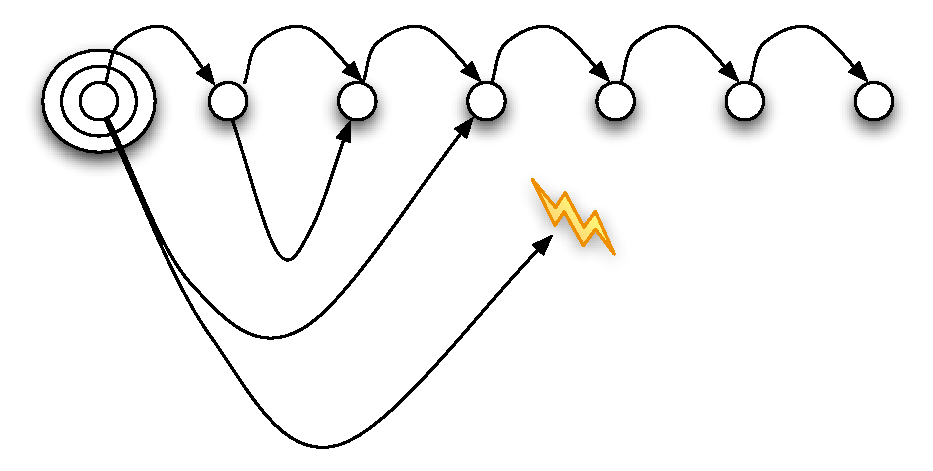
\includegraphics[width=0.75\linewidth]{figures/dedalus-time.pdf}
%   \label{fig:time}
%   %%\caption{Time moves forward in three ways: across strata, to the next fixpoint, and to some future fixpoint.}
%    \caption{Dedalus admits inferences whose consequences are visible immediately, in the next timestep, or at some unspecified timestep.}
%    
% \vspace{-8pt}
% \end{figure}

Until now we have restricted our discussion to \slang.  In this section we
introduce \lang, a superset of \slang that also admits aggregate functions
and the \emph{choice} construct.  These constructs will allow us to
express programs that establish or enforce an ordering over inputs, and to
reason about the inherent nondeterminism in communication over unreliable
networks that may delay, lose or reorder the results of logical deductions. 
%(see Figure~\ref{fig:time}).

\subsection{{\bf \large \lang}: New Constructs}

In this section we present the Datalog extensions missing from \slang that we will need in \lang to capture important properties of practical distributed systems.  These include aggregate functions to 
capture ordering constraints, and---more importantly---the choice construct to capture nondeterminacy.

\subsubsection{Aggregate Functions}
Mumick and Shmueli observe correspondences in the expressivity of Datalog with stratified negation and stratified aggregation functions~\cite{mumickshmueli}.  Adding aggregation to our language does not affect its expressive power, but is useful for writing natural constructs for distributed computing including queues and ordering.  

In \lang we will allow
aggregate functions $\rho_1 - \rho_n$ to appear
in the head of a deductive rule of the form:

\dedalus{p(\(A_1\), \(\ldots\), \(A_n\), \(\rho_1\)(\(A_{n+1}\)), \(\ldots\), \(\rho_m\)(\(A_{n+m}\))) \(\leftarrow\)}
\linebreak\dedalus{\(q_1\)(\(A_1\), \(\ldots\), \(A_n\)), \(\ldots\), \(q_n\)(\(A_1\), \(\ldots\), \(A_n\));}

According to this rule, the predicate $p$ contains one row for each satisfying assignment of $A_1, \ldots, A_n$ -- akin to the distinct ``groups'' of SQL's ``GROUP BY'' notation.

% These functions do not affect the expressivity of the language; we admit them
% to simplify our discussion of ordering.  It is easy to see that the \emph{min} function,
% which we subsequently use, is expressible in Datalog using negation.

%%\begin{example}
%%The query below selects, for each distinct value of the first column of $p$, the minimum 
%%value of the second column.

%%\begin{Dedalus}
%%min_p(A, min<B>) \(\leftarrow\) p(A, B);
%%\end{Dedalus}

%%The Datalog program below is equivalent:

%%\begin{Dedalus}
%%notmin_p(A, B) \(\leftarrow\) p(A, B), p(A, C), B > C;
  
%%min_p(A, B) \(\leftarrow\) p(A, B), \(\lnot\)notmin_p(A, B);
%%\end{Dedalus}
%%\end{example}




%%\dedalus{r\pos($A_1$, $A_2$, [...], $A_n$, }

%%$\rho$($A_{n+1}$)}

%%$\rho$($A_{n+2}$), [...] $\rho$($A_{n+m}$)) \(\leftarrow\) r($A_1$, $A_2$, [...], $A_n$);}



\subsubsection{Choice}
A signature feature of distributed systems is that individual computers cannot control or observe the temporal interleaving of their computations with other computers.  One aspect of this uncertainty is captured in network delays: the arrival ``time'' of messages cannot be directly controlled by either sender or receiver.  In this section, we enhance our language with a traditional model of non-determinism from the literature to capture these issues: the \emph{choice} construct as defined by Greco and Zaniolo~\cite{greedychoice}.

The subgoal \dedalus{choose((\emph{$X_1$}), (\emph($X_2$))} may appear in the body of a rule, where
\emph{$X_1$} and \emph{$X_2$} are vectors whose constituent variables occur elsewhere in the body.  Following Greco and Zaniolo, such a subgoal
enforces the functional dependency \emph{$X_1$} $\to$ $X_2$, ``choosing" a single assignment of values to the variables
in \emph{$X_2$} for each variable in \emph{$X_1$}.

The choice construct is nondeterministic.  In a model-theoretic interpretation of logic programming, a nondeterministic program 
must have a multiplicity of stable models -- that is it must be unstratifiable.  Greco and Zaniolo define 
choice in precisely this fashion: the choice construct is expanded into an unstratifiable strongly connected component of rules, 
and each possible choice is associated with a different model.

\paa{significantly, for any choice, the resulting program has a unique minimal model if the program (independent of the choice expansion)
is stratifiable, locally stratifiable, etc}  \jmh{You do need to resolve the previous paragraph, or rewrite it to simply say ``see the Italians if you want to understand more, but for our purposes assume a unique non-deterministic assignment that respects the FDs.  This allows us to have agreed-upon minimal models.''}

\subsection{Distribution Model}

A principal motivation for \lang is to model and implement distributed systems.
To represent a distributed system, we consider a some number of
agents; each running a {\em subprogram} that consists of some subset
of the relations referenced by the \lang program running on the
distributed system.  We constrain the \lang rules so that each rule's
body ontains predicates from exactly one subprogram.  The head of
asynchronous rules may reference a relation in any subprogram, but the
head of all other rules must reference a relation in the subprogram
that contains the predicates in the body.  Rules that span subprograms are
{\em communication rules}.

This restricts communication between nodes in two important ways.
First, by restricting bodies to a single agent, it forces all
communication between agents to be via communication rules.  Second,
because all communication rules are asynchronous, agents may only
learn about time values at another agent by receiving messages (with
unknown delay) from that agent.  Note that this model says nothing
about the relationship between the agents' clocks; they could be
non-monotonically increasing, or they could respect a global order.
We now turn to a discussion of such constraints.

\subsection{Asynchronous Rules}

In order to represent the nondeterminism introduced by distribution, we admit a
third type of rule, called an {\em asynchronous} rule.  A rule is asynchronous
if the 
%Recall our use of the distinguished variables $\Tau$ and $S$ to represent the
%time suffixes respectively in the body and head of a rule
%(Section~\ref{sec:syntaxrestrictions}).  in our discussion of \slang,
%representing the time suffixes occuring respectively in the body and head of a
%rule.
relation between the head time suffix $\SDedalus$ and the body time suffix $\Tau$ is
unknown.  Furthermore, $\SDedalus$ (but not $\Tau$) may take on the special value
$\top$ which means ``never.''  Derivation at $\top$ indicates that the
deduction is ``lost,'' as time suffixes in rule bodies do not range over
$\top$.

We model network nondeterminism using the \dedalus{choice} construct to choose
from a value in the special 
%%\dedalus{successors} 
\dedalus{time}
predicate, which is defined using the following datalog rules:

\begin{Dedalus}
time(\(\top\));
time(\(\SDedalus\)) \(\leftarrow\) successor(\(\SDedalus\), _);
\end{Dedalus}

\noindent
Each asynchronous rule with head predicate \dedalus{p($A_1, \ldots, A_n$)} has the following additional subgoals in its
body: \dedalus{time($\SDedalus$), choose(($A_1, \ldots, A_n, \Tau$), ($\SDedalus$))}, where
$\SDedalus$ is the timestamp of the rule head.  Note that our use of \dedalus{choose} incorporates all variables of each head predicate tuple, which allows a unique choice of $\SDedalus$ for each head tuple.


\begin{example}
A well-formed asynchronous \lang rule:

\begin{Dedalus}
r(A, B, \(\SDedalus\)) \(\leftarrow\) 
  e(A, B, \(\Tau\)),
  time(\(\SDedalus\)), choose((A, B, \(\Tau\))), (\(\SDedalus\)));
\end{Dedalus}
\end{example}

We admit a new temporal head annotation to sugar the rule above.  The
identifier \dedalus{async} implies the rule is asynchronous, and stands in for
the additional body predicates.
%%$N$ is a variable,
%%corresponding to the time suffix $\Tau$ of all predicates in the rule body and
%%optionally referenced in the head.  
The above example expressed using \dedalus{async} is:

% asynchronous
\begin{example}
	A sugared asynchronous \lang rule:
	
\begin{Dedalus}
r(A, B)@async \(\leftarrow\) e(A, B);
\end{Dedalus}
\end{example}


\subsubsection{Later: Causally-Constrained Asynchrony}


\jmh{What do we need here?  We need to resurrect safety and strat for \lang, not just for \slang.  Monotonic deductive reductions are always cool.  Non-monotonic ones need us to ``inject'' monotonicity via the time suffix.  We lost this with async (which is natural in distributed systems).  We regain it via the addition of rules to enforce monotonicity -- these are akin to Lamport clocks and have the nice property that they don't ``cheat'', they follow our rules on messaging and asynchrony.}

Nothing in our definition of asynchronous rules prevents tuples in the
head of a rule from having a timestamp $\SDedalus$ that is less than
$\Tau$, the timestamp in the rule's antecedents. This is a significant
departure from \slang, since it violates the monotonicity assumptions
upon which we based our proof of temporal stratification.  On an
intuitive level, it may also trouble us that rules can derive head
tuples that exist ``before'' the body tuples on which they are
grounded; this violates intuitive notions of ``causality.''  Consider
the following program, which exihibits non-determinism in the face of
executions that violate causality:

\begin{Dedalus}
r(1)@1;
s(1)@2;
p(X) \(\leftarrow\) q(X), r(X);
q(X)@async \(\leftarrow\) s(X);
\end{Dedalus}

Since \dedalus{s(1)} and therefore \dedalus{q(1)} are derived after
\dedalus{r(1)} ceases to exist, it seems unreasonable that
\dedalus{@async} leads to schedules where the join of \dedalus{q(1)}
and \dedalus{r(1)} succeeds.

Ideally, we would like \lang to have safety and stratifiablity
propertes similar to those of \slang.  An examination of the proofs
\rcs{which I have not performed, and am speculating about} reveals
that the main deficiency in \lang's semantics are due to its
abandonment of monotonically increasing timesteps.

The solution is simple; rather than define \dedalus{time}, we define a relation \dedalus{after}:

\begin{Dedalus}
after(S, T) \(\leftarrow\) successor(S, T);
after(S, U) \(\leftarrow\) after(S, T), successor(T, U);
after(S, \(\top\)) \(\leftarrow\) successor(S, _);
\end{Dedalus}

and, as above, we define the sugar \dedalus{@later}, which adds the
following predicates to rule bodies:

\begin{Dedalus}
after(\(\Tau\), S),
choose((\(A_1, \ldots, A_n, \Tau\)), (S))
\end{Dedalus}

We call the resulting language \lang$_{late}$


\begin{lemma}
Lemmas~\ref{lemma:no-neg-unique} and~\ref{lemma:temp-strat-uniq} apply
to \lang$_{late}$ up to choice.
\begin{proof}
We need to show that, given an assignment of values by
\dedalus{choose}, we have unique minimal models.  Here is a proof
sketch.  The only timestamp related assumption made by
Proofs~\ref{lemma:no-neg-unique} and~\ref{lemma:temp-strat-uniq} is
that timestamps increase monotonically over time.  The definition of
\dedalus{after} ensures that \dedalus{choose} selects such a value, in
which case the proof holds, or $\top$, which leads to lost deductions,
which cannot introduce cycles.
\end{proof}
\end{lemma}

Thus, although \lang$_{late}$ is, by definition, non-deterministic, any given evaluation of a \lang$_{late}$ program has semantics analgous to \slang.

This restores the monotonicity properties relied upon by
Lemmas~\rcs{XXX???} which hold over \lang with \dedalus{@later}, but
not with \dedalus{@async}.

Ultimately, whether a particular set of temporal semantics is
desirable depends on the underlying application.  For example, many simple distributed applications ``don't care'' about ordering of events, assuming that users can tolerate out-of-order semantics as long as things accumulate monotonically.  The standard example in recent years is in web discussion boards, where comments on articles may appear ``out of order'' on the board for some users: that is, a response to some comment may appear before the comment itself appears.  This typically happens because the discussion board is actually a distributed system with replication of the content across sites, and the transmission of replicated data does not observe a causal ordering.

%%\rcs{move this, get rid of monotonic discussion?
%%We observe, however, that the order of evaluation of a Datalog program is irrelevant to the final result when the program is 
%%purely monotonic.  For such a program~\footnote{This holds also for the trivial cases of programs that ignore messages.}, 
%%deductions ``into the past" present no difficulties.
%%In fact, the ``eventual consistency" property of NDLog~\cite{loo-sigmod06} relies on the assumption that
%%programs are negation-free and hence monotonic.  Any programs with non-monotonic rules that transitively depend on
%%message tuples, however, may need to enforce an ordering discipline on such tuples.  We discuss this in detail in Section (Lamport Clocks).
%%}

The distributed systems literature often requires a causal ordering
of events across systems; Lamport clocks~\cite{lamportclock} are a simple mechanism go achieve this.  Lamport clocks
record the partial ordering induced by network communication between
the nodes.  With such approaches in mind, we introduce an alternative
to \dedalus{@async} called \dedalus{@later} that induces a total
ordering over all timestamps within a \lang program.  We define \dedalus{after} as the transitive closure of \dedalus{successor} including $\top$:


Intuitively, \dedalus{after(S, T)} is true if T happens after S in the
global ordering of events.  Each rule \dedalus{p($A_1, \ldots, A_n$)@later} has the
following additional variables in its body:
\dedalus{after($\Tau$, S),} \\
\dedalus{choose(($A_1, \ldots, A_n, \Tau$), (S))}, where, as
above, $\Tau$ is the timestamp associated with the rule body, and
\dedalus{S} is the timestamp of the rule head.

Note that our addition of a global ordering does not expose a shared
synchronized clock to \lang programs.  The nondeterminism associated with
choice prevents programs from ensuring that operations are performed in
lock-step.  Instead, the timestamps simply encode some logical clock that is
equivalent to one that could be maintained by the application.  The difference
is that, by constraining \dedalus{choose}, we can avoid reasoning about program
traces that contain paradoxes such as causality loops.  In particular,
deterministic instances such as:

are non-deterministic if \dedalus{@later} is replaced with
\dedalus{@async}.  
\paa{the rest may stay but may also go}
The non-determinism comes from \dedalus{@sync}'s
\dedalus{choose} invocation.  However, the non-determinism also relies
on the fact that the program is, in some sense, non-monotonic; it
relies on the fact that \dedalus{r(1)} stops being true before
\dedalus{q(1)} is derived.

%%\rcs{Can we prove anything now?  It seems as though async rules are equivalent to \slang rules, as long as there is no aggregation or arithmetic.  The problem is that if %%choice derives a fact N steps in the future, we need to push the fact through N @next rules, and the number of such rules is variable.  If we admit arithmetic in the rewrite, %%%we can model async as a synchronous queue, but \slang doesn't have arithmetic...}
%%\rcs{Here to end of section is dead text}





%\dedalus{time(t)} is true if $t \in \mathbb{Z} \cup \top$. 
%%\rcs{didn't understand the $\Theta$ thing; kill this paragraph?}
%%An asynchronous rule has the following
%%subgoals in its body: \dedalus{time(S), successors($\Theta$, S), choose(($\Theta$), (S))}, where
%%$\Theta$ is a vector containing all variables appearing in the rule body,
%%including $\Tau$.  The choice subgoal expresses that the rule head may be
%%derived at any value of \dedalus{time}.
%time value that appears in the \dedalus{successor} relation.

%%\rcs{old example:}

%%\begin{Dedalus}
%%asynchronous
%%r(A, B, S) \(\leftarrow\)
%%   e(A, B, \(\Tau\)), successor(_, S), choose((A, B), (S));
%%\end{Dedalus}


\subsubsection{Entanglement}

Consider the asynchronous rule below:

\begin{Dedalus}
p(A, B, N)@async \(\leftarrow\)
  q(A, B)@N;
\end{Dedalus}

Due to the async keyword in the rule head, each \emph{p} tuple will take some unspecified time suffix value.
Note however that the time suffix $N$ of the rule body appears also in an attribute of \emph{p} other than the time suffix, recording a 
binding of both the time value of the deduction and the time value of its consequence.  We call such a binding
an \emph{entanglement}.   Entanglement is a surprisingly powerful construct that allows a rule to 
reference the logical clock time of the deduction that produced one (or more) of its subgoals.  Note that in order
to write the rule it was necessary to not sugar away the time suffix in the rule body.  We restrict the use of entanglements to asynchronous rules. \jmh{Why the restriction?  Also, can you justify that it's surprisingly powerful?}

\jmh{Where do we give the def that say ``\lang is \slang with the following extra goo''?  Here?  After async?}

\subsection{Ordering and distribution in Logic}

\subsubsection{Sequences}
\jmh{I fixed this so it can be done entirely in \slang.  Move it forward as you see fit, or comment here that it's plain old \slang but you mention it now for some reason.}
One may represent a database sequence---an object that retains and monotonically increases a counter value---with a pair of inductive rules.  One rule increments the current counter value when some condition is 
true, while the other persists the value of the sequence when the condition is false.  We can capture the increase
of the sequence value without using arithmetic, because the infinite series of \emph{successor} has the monotonicity
property we require:

\begin{Dedalus}
seq(B)@next \(\leftarrow\) seq(A), successor(A,B), event(_).
  
seq(A)@next \(\leftarrow\) seq(A), \(\lnot\) event(_);
\end{Dedalus}

Note that these two rules produce only a single value of seq at each timestep, but they do so in a manner slightly different than our standard persistence template.
%%We must admit arithmetic functions into our language to express such a
%%sequence, but the pair of rules above remains temporally safe.

% Clearly, to implement a sequence that increases consecutively without gaps would require using arithmetic.


\subsubsection{Queues}
\jmh{Motivate me!}

\jmh{Notice again -- no entanglement, no async.  Just aggs.  Could be in \slang if you would admit aggs into \slang (and why wouldn't you?)}
%%Consider a trace of events to a 

\jmh{Can't we whittle this down to the bone?  Why are we dealing with user and job attributes?  Why not drop user?}Consider a predicate \dedalus{priority\_queue} that represents a series of tasks to be performed in some predefined order.  Its attributes are a string representing a user, a job, and an integer
indicating the priority of the job in the queue:

\begin{Dedalus}
priority\_queue(``bob'', ``bash'', 200)@123;
priority\_queue(``eve'', ``john'', 1)@123;
priority\_queue(``alice'', ``ssh'', 204)@123;
priority\_queue(``bob'', ``ssh'', 205)@123;
\end{Dedalus}

Note that all the time suffixes are the same.  
%Depending on the program that implements the balance update, several behaviors
%are possible.
Given this schema, we note that a program would likely want to process
\dedalus{priority\_queue} events individually in a data-dependent order, in
spite of their coincidence in logical time.  It is difficult to express general
in-order tuple processing in Datalog, in part because the language does not
admit sequences.  \jmh{Huh?  I don't see the last clause there.  Maybe say simply that Datalog is set-oriented, but what we want here is precisely to impose an ordering on the elements of the set, which seems unnatural.  There's maybe a connection to expressibility and aggregation or arithmetic or something, but let's not try to sort that out for now.}
%above is really what we want to say, right? -wrm
%has so
%notion of order of evaluation (except the implicit ordering implied by
%stratification).

In the program below, we define a table \dedalus{m\_priority\_queue} that
serves as a queue to feed \dedalus{priority\_queue}.  The queue must persist
across timesteps because it may take multiple timesteps to drain it.  At each
timestep, for each value of \textbf{A}, a single tuple is projected into
\dedalus{priority\_queue} and deleted (atomic with the projection) from
\dedalus{m\_priority\_queue}, changing the value of the aggregate calculated
at the subsequent step:

\begin{Dedalus}
% persist m\_priority\_queue
m\_priority\_queue(A, B, C)@next \(\leftarrow\)
  m\_priority\_queue(A, B, C),
  notin del\_m\_priority\_queue(A, B, C);

% find the min priority
omin(A, min<C>) \(\leftarrow\)
  m\_priority\_queue(A, _, C);

% feed p in the next step 
% with the items of min priority
p(A, B, C)@next \(\leftarrow\)
  m\_priority\_queue(A, B, C),
  omin(A, C);

% delete from the next step 
% those items of min priority
del\_m\_priority\_queue(A, B, C) \(\leftarrow\)
  m\_priority\_queue(A, B, C),
  omin(A, C);
\end{Dedalus}

Under such a queueing discipline, deductive rules that depend on
\emph{priority\_queue} are constrained to consider only min-priority tuples at each timestep
per value of the variable \textbf{A}, thus implementing a per-user FIFO
discipline.  To enforce a global FIFO ordering over \emph{priority\_queue}, we
may redefine \emph{omin} and any dependent rules to exclude the \textbf{A}
atttribute.

\jmh{This paragraph is a bit of a mouthful.  And didn't we say this already?}
A queue establishes a mapping between the local clock and the priority-ordering attribute of the input relation. By doing so, we are able to take
advantage of the natural ordering enforced by stratification over time, to enforce an ordering property over our input that is otherwise 
very difficult to express in a logic language.

\subsubsection{Lamport Clocks}
Recall that \dedalus{@async} provides weaker semantics than
\dedalus{@later}, and can even lead to program executions that violate
causality.  In contrast, \dedalus{@later} builds a number of
assumptions about time into the language model.  This section explains
how to implement Lamport clocks~\cite{timeclocks} atop
\dedalus{@async}, ensuring that the program observes a causal ordering
of events.  Depending on the runtime environment, making use of
\dedalus{@async} and explicitly maintaining Lamport clocks may be more
or less natural than \dedalus{@later}.  \jmh{Any plan of convincing me of the pros and cons of these?  I'd say they're the same, and you should toss out later?}

Consider a rule \dedalus{p(A,B)@async \(\leftarrow\) q(A,B)}.  By
rewriting it to:

\begin{Dedalus}
persist[p, 2]
p\_wait(A, B, N)@async \(\leftarrow\) q(A, B)@N;
p\_wait(A, B, N)@next \(\leftarrow\) p\_wait(A, B, N)@M, N \(\ge\) M;
p(A, B)@next \(\leftarrow\) p\_wait(A, B, N)@M, N < M;
\end{Dedalus}

we place the derived tuple in a new relation \dedalus{p\_wait} that
stores any tuples that were ``sent into the past'' until the point in
time at which they were derived.  Conceptually, this causes the system
to evaluate a potentially large number of timesteps (if N is
significantly less than the timestamp of the system when the tuple
arrives).  However, if the runtime is able to efficiently evaluate
timesteps when the database is quiescent (by recognizing that the
timesteps can be skipped, as is done in Algorithm~\ref{alg:tsn}), then instead of ``waiting'' by evaluating
timesteps, it will simply increase its logical clock to match that of
the sender.  In contrast, if the tuple is ``sent into the future,''
then it is processed using the timestep that receives it.  This
manipulation of timesteps and clock values is equivalent to
conventional descriptions of Lamport clocks.

\jmh{Can't we please do the normal use of Lamport clocks, i.e. show how it solves a distributed systems problem?}


